\chapter{Background}

% TODO:
% Talk about:
%  * DBMS.
%  * Isolation levels.
%  * Fuzzing.
 
\section{Database Management Systems}

Modern database management systems (DBMS) are complex software systems that provide a high-level interface for users to interact with the underlying data. DBMSs such as \textit{MySQL} \cite{mysqlwebpage} offer a large set of features, including data storage, retrieval and manipulation.

Relational DBMSs, usually exposing \textit{SQL} as a query language, form an overwhelming majority of the database systems in use today, with the 4 most popular DBMSs being relational \cite{akhtar2023popularity}. The relational model was introduced by Edgar Codd in $1970$ \cite{codd1970relational}, and offers application developers a high-level manipulation capacity of the stored data. Information is modeled as collections of relations between properties, commonly represented as tables and rows.

Modern \textit{SQL} offers a \textit{Data Definition Language} (DDL) to create and modify the structure of the underlying data, and a \textit{Data Manipulation Language} (DML) to interact with the data. The DDL is composed of statements such as \textit{CREATE} and \textit{DROP}, while DML is composed of statements such as \textit{SELECT}, \textit{INSERT}, \textit{UPDATE}, and \textit{DELETE}.

\section{Transactions}

A transaction is a sequence of instructions executed as a single isolated unit of work. In other words, either all of the instructions in the transaction are correctly executed and saved to the database, or none of them are. Transactions offer the ACID properties \cite{gray1981transaction}, a set of properties that guarantee that database transactions are processed reliably. The ACID properties are as follows:

\begin{itemize}
    \item \textbf{Atomicity}: A transaction is an atomic unit of work, meaning that the database will either execute all of the instructions in the transaction, or none of them.
    \item \textbf{Consistency}: A transaction will bring the database from one consistent state to another consistent state. In other words, the database will always be in a consistent state, regardless of the state of the running transactions.
    \item \textbf{Isolation}: Multiple transactions can be executed concurrently, and, depending on the isolation level, the transactions will not interfere with each other.
    \item \textbf{Durability}: Once a transaction is committed successfully, the DBMS guarantees that the changes made by the transaction will be saved to the database.
\end{itemize}


\section{Isolation Levels}

The isolation between transactions is defined by the isolation level. Stricter isolation levels offer more consistency guarantees, at the cost of concurrency and performance. While many isolation levels have been formalized, the ANSI isolation levels supported by most database systems \cite{melton1992iso_ANSI} are as follows:

\begin{itemize}
    \item \textbf{Read Uncommitted}: The lowest isolation level. Transactions can read uncommitted data from other transactions.
    \item \textbf{Read Committed}: Transactions are visible only after being committed.
    \item \textbf{Repeatable Read}: Transactions are visible only after being committed, and multiple reads of the same data will return the same result. Note that new data can be become visible to the transaction.
    \item \textbf{Serializable}: The strongest (and slowest) isolation level, in which transactions can be assumed to be executed serially.
\end{itemize}

% Add the image `assets/adya_isolation_levels.png`.
\begin{figure}[H]
    \centering
    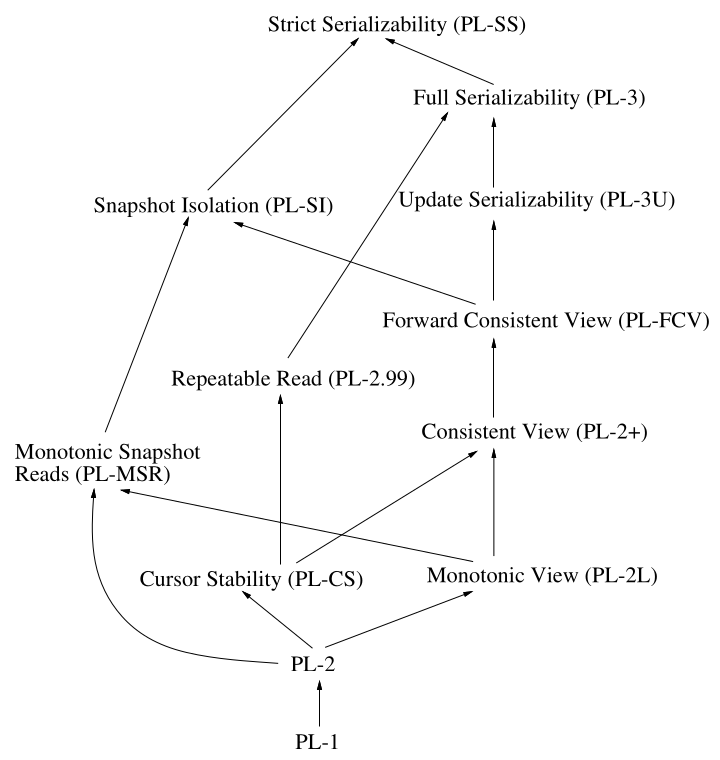
\includegraphics[width=0.7\textwidth]{assets/adya_isolation_levels.png}
    \caption{The Adya isolation levels \cite{adya1999weak}.}
    \label{fig:adya_isolation_levels}
\end{figure}

In modern DBMSs, the isolation levels are implemented by leveraging concurrency control techniques such as locking and multi-version concurrency control (MVCC). The choice of isolation level is a trade-off between consistency guarantees and concurrency performance, and is usually made by the application developer.

For instance, a banking application which needs to avoid double-spending will use the \textit{Serializable} isolation level, while a school grading system might want to use the \textit{Read Committed} isolation level.

\section{Transaction and Isolation Bugs}

DBMSs are complex software systems, with their complexity constantly increasing as diminishing returns push for more and more complex optimizations. Like all software, DBMSs are prone to bugs, which can lead to data corruption, loss of data, or crashes.

Transaction and isolation bugs are part of a specific class of bugs residing in the transaction and isolation handling mechanisms of a DBMS. Such bugs are tricky to detect, as they often require multiple concurrent transactions, might occur sporadically due to the nondeterministic nature of the concurrency, and might not be easily reproducible.

While similar, transactional and isolation bugs are slightly different:
\begin{itemize}
    \item \textbf{Transactional bugs}: Logic bugs that occur when one or multiple transactions are being run. Possible manifestations include unexpected failures, missing data, or incorrect behavior.
    \item \textbf{Isolation bugs}: Bugs that occur when the specified isolation level is not respected. Possible manifestations include forbidden behavior, such as dirty reads, non-repeatable reads, or phantom reads.
\end{itemize}

\section{Related Work}

The topic of database testing is not new, with multiple techniques and tools being developed over the years. Recent work has focused on fuzzing techniques, combined with novel methods of detecting errors in random transactions \cite{jiang2023detecting, cui2022differentially_ASE2022, dou2023detecting_ICSE2023, clark2024validating}. A recent paper by Cui, Z.\ et al. \cite{cui2024understanding_ICSE2024} makes a comprehensive survey of reported transactional bugs, a large portion discovered with the help of the before-mentioned fuzzing techniques.

Our work is inspired by the surveying work of Cui, Z.\ et al. \cite{cui2024understanding_ICSE2024}, and aims to replicate and analyze bugs, by providing an easy way to test them. In the best of our knowledge, the authors of the survey did not actually replicate the collected bugs, due to constraints on the DBMS versions (often a Git commit) and time consumption, and relied on the original bug reports instead.

In the second part of our project, we also build on the work of Clark, J. et al. \cite{clark2024validating} which find bugs by checking violations of the Adya dependency graph \cite{adya1999weak} in a white-box fashion, and on the work of Jiang, Z. et al. \cite{jiang2023detecting} which introduces the novel idea of SQL instrumentation. Using these two techniques, we introduce a new technique for finding isolation bugs using Adya dependency graphs in a black-box fashion, leveraging the SQL instrumentation technique.

% % BELLOW NOT WRITTEN BY ME, OLD PROJECT
% \section{Consistency Models}


% Consistency models are a fundamental concept i n distributed systems. We will briefly describe some definitions here. Most of the definitions can be found in \cite{Consiste95:online}. First, we define distributed systems as a collection of processes and a system of states. Note that the process and the state here are purely logical and can be abstracted from the actual computer concepts.

% A process is single-threaded and could only do one thing at a time. Processes communicate via the network, and the communication is asynchronous. The system state is a set of key-value pairs. The operation is a step taken at some process. It can be reading an item, writing to an item, or sending a message. A history is a collection of the operation and the system state. The concurrency control level defines which set of history is legal.
% \subsection{Strict Serializability}
% Strict Serializability is the most strict level of concurrency control. The transactions must form a total order. The net effect is that the transaction could not be interleaved with each other. And that total order must be consistent with the real-time order. Strict serializability implies serializability and linearizability. 
% \subsection{Causal Consistency}
% Causal consistency captures the notion that causally-related operations should appear in the same order across all processes. Processes may however disagree about the order of causally independent operations.

% The causal relationship comes from Lamport's happen-before relationship. If two operations happen on the same processor, they have causal relationships and are consistent with the real-time order. If two operations have a send-receive relationship, they are also considered causal. For example, a message $A$ sent at processor $X$ and received at processor $Y$ is also considered to have a causal relationship.






% \subsection{Snapshot Isolation}
% In snapshot isolation, each transaction appears to operate on an independent state of the system, and this independent state is called a snapshot. In other words, If transaction $T_1$ has modified an object $x$, and another transaction $T_2$ committed a write to $x$ after $T_1$’s snapshot began, and before $T_1$’s commit, then $T_1$ must abort. 
% \section{Impossibility Results}
% Consistency models require systems to adhere to some requirements. The concurrent control algorithms are practical protocols to ensure that the process following the protocols will adhere to the consistency models. Due to the constraint of requirements of the consistency models, some impossibility results are established to help people understand what can be achieved and what can not be achieved. Here we discuss three important impossibility results. 
% \subsection{SNOW}
% First, we will discuss the SNOW theory. The SNOW theory states that the following four properties cannot be achieved at the same time.
% \begin{enumerate}
%     \item \textbf{S}: Strict Serializability.
%     \item \textbf{N}: Non-blocking operation.
%     \item \textbf{O}: One response per read.
%     \item \textbf{W}: Write Transactions that conflict.
% \end{enumerate}

% We will discuss these four properties in more detail.


% \textbf{S} stands for strict serializability.

% \textbf{N} stands for non-blocking operation. This means that each operation inside a read-only transaction could not be blocked by an external event such as a lock. 
% \textbf{O} stands for one response per read. This means two things. First, when the server issues a read, it will only incur one round trip of read. In other words, no retry of reading is allowed. Second, only one version of the read result is allowed to return. This means that the server can only return one version of the data. 

% \textbf{W} stands for write transactions. This property requires that the write transactions can co-exist in the distributed system with the read-only transactions. In other words, the system can allow both read-only transactions and write-only transactions.

% \cite{lu2016snow} states the SNOW properties as follows.
% \textit{No read-only transaction algorithm provides all of the SNOW properties}. In other words, there does not exist a distributed system or concurrency control algorithm that satisfies all of the SNOW properties.


% \subsection{NOCS}
% Next, we will also introduce the \textbf{NOCS} impossibility result. \textbf{NOCS} is based on the \textbf{SNOW} impossibility result. Like \textbf{SNOW}, \textbf{NOCS} also defines four properties.

% \begin{enumerate}
%     \item \textbf{N}: Non-blocking execution.
%     \item \textbf{O}: One-round communication.
%     \item \textbf{C}: Constant meta data.
%     \item \textbf{S}: Strict Serializability
% \end{enumerate}

% \paragraph{Understanding NOCS}
% Unlike \textbf{SNOW}, \textbf{NOCS} focuses on optimal performance. Theoretically speaking, concurrency control has to pay attention to both the local computation time and the network communication time to achieve optimal performance. The shortest local computation time the process can take is in a non-blocking execution fashion (we are only talking about the theory results here, so we ignore practical issues such as the hardware performance). The network communication time depends on the following factors: the round of communication and the payload itself. The minimum number of rounds of communication is one, and the payload has to at least include the data itself and possibly with constant metadata (again, we are also ignoring practical factors such as the network speed and are only focusing on the theory framework). That is to say, to achieve the theoretically best result, a concurrency control has to satisfy the following three properties.

% \begin{enumerate}
%     \item The local computation side has to be a non-blocking execution.
%     \item The network side only includes one round of communication.
%     \item The network side only transfers necessary data: the data itself and the constant size metadata. 
% \end{enumerate}

% These three properties are exactly what \textbf{NOC} stands for.


% Next, we will state the \textbf{NOCS} theorem.

% \paragraph{NOCS Theorem} Performance-optimal read-only transactions cannot provide strict serializability. In other words, there does not exist a concurrency control algorithm that satisfies \textbf{NOCS} together.




% \subsection{NOC-NOC}

% The above two impossibility results only focus on read-only transactions. Although read-only transactions are widely found in most workloads \cite{cooper2010benchmarking}, as the YCSB workload shows \cite{cooper2010benchmarking}, some of the workloads are also dominated by write.  \textbf{NOC-NOC} is based on \textbf{NOC} and is intended also to consider the performance of write transactions.


% The first three \textbf{NOC} consider the read-only transactions' performance.


% \begin{enumerate}
%     \item \textbf{N}: Non-blocking reads. 
%     \item \textbf{O}: One-round trip reads.
%     \item \textbf{C}: Constant-size meta-data for reads.
% \end{enumerate}


% The first \textbf{N} requires that when a read operation happens, it does not have to wait for an external event such as a lock acquire or a lock release. The second \textbf{O} requires that when a read happens, only one round of communication is enough. The third \textbf{C} requires that only constant size meta data plus the data itself is allowed to be transferred via the network.

% The second three \textbf{NOC} consider the write-only transactions' performance.


% \begin{enumerate}
%     \item \textbf{N}: Non-blocking write.
%     \item \textbf{O}: One-phase write.
%     \item \textbf{C}: Constant-sized meta data for write.
% \end{enumerate}


% The second \textbf{N} requires that the write operation has also to be non-blocking, i.e., without waiting on external events such as lock release. This excludes common concurrency control algorithms such as distributed locking. The second \textbf{O} requires that there should only be one-phase write, meaning that the write will happen asynchronously. The second \textbf{C} means that, in the same way as read, the metadata size of should be constant besides the actual data size.



% \paragraph{NOC-NOC Theorem} 
% The \textbf{NOC-NOC} theorem states the following: \textit{No transactions algorithms that support parallel snapshot isolation or snapshot isolation concurrency control level could satisfy all \textbf{NOC-NOC} properties}.

